\documentclass[conf]{new-aiaa}
%\documentclass[journal]{new-aiaa} for journal papers
\usepackage[utf8]{inputenc}

\usepackage{graphicx}
\usepackage{amsmath}
\usepackage[version=4]{mhchem}
\usepackage{siunitx}
\usepackage{longtable,tabularx}
\usepackage{algorithm}
\usepackage{algorithmic}
\setlength\LTleft{0pt} 


\title{Modifying Scheduled Flight Paths to Track the Motion of Regular Traffic}

\author{Leonardo Pi{\~{n}}ero-P{\'{e}}rez\footnote{Engineer I, Flight Control Laws, leonardo.pinero42@gmail.com, AIAA Member.}}
\affil{Bell Flight, Arlington, TX, 76019}

\begin{document}

\maketitle

\begin{abstract}
Insert Abstract Here. It should be one paragraph long (not an introduction) and complete in itself (no reference numbers). It should indicate subjects dealt with in the paper and state the objectives of the investigation. Newly observed facts and conclusions of the experiment or argument discussed in the paper must be stated in summary form; readers should not have to read the paper to understand the abstract. The abstract should be bold, indented 3 picas (1/2'') on each side, and separated from the rest of the document by blank lines above and below the abstract text.
\end{abstract}

\section{Nomenclature}

{\renewcommand\arraystretch{1.0}
\noindent\begin{longtable*}{@{}l @{\quad=\quad} l@{}}
$\alpha$ & hyperparameter to determine tuning update \\
$\beta$  & tuned scaling parameter \\
$\delta$ & scaling vector for alteration vector \\
$\eta$ & mutation factor \\
$\lambda$ & hyperparameter for determining total cost \\
$\mu$ & tuned value of symmetry for shaping \\
$\theta$ & angle between distance vector and simulated object path \\
$\rho$ & tuned power-scaling bias \\
$\sigma$ & tuned standard deviation parameter of activation function \\
$b$ & index of child set of parameters \\
$B$ & batch size \\
$C$ & cost metric for a given flight path \\
$\vec{d}$ & distance vector from node to anchor point\\
$e$ & denotes last ``known'' point location (last anchor point) for simulated object point \\
$i$ & iteration of an initial or altered path \\
$I$ & total number of main loop iterations \\
$j$ & index of a node for a given path leg \\
$k$ & index of a contacted object point \\
$K$ & set of $k$ contacted object points \\
$\vec{n}$ & node location \\
$\vec{o}$ & target object location \\
$P$ & tracking performance for a given flight path \\
$\mbox{randn}(B)$ & outputs $B$ normally distributed random numbers with a mean of 0 and standard deviation of 1 \\
$s$ & denotes first ``known'' point location (first anchor point) for simulated object path \\
$t$ & location along time axis \\
$T$ & discretized locations along time axis representing a section of the path's flight time \\
$\vec{u}$ & orthonormal basis vector for the planes of alteration \\
$x$ & location along East/West axis \\
$X$ & discretized locations along East/West axis representing a path section \\
$y$ & location along North/South axis \\
$Y$ & discretized locations along North/South axis representing a path section \\
\end{longtable*}}

% ====================================================================
% INTRODUCTION
% ---------------------
% ====================================================================
\section{Introduction}
A methodology for tracking moving objects with an existing fleet of aircraft is developed. An ``object'' is defined as any detectable information moving spatially as a \emph{cyclical} function of time, such as automobile traffic for a given weekday, other aircraft on a given schedule, or air pollution for a given a week. In real-world applications, a fleet of unmanned aerial vehicles is the intended platform for obtaining measurements. The approach provides:
\begin{enumerate}
\item Operational flexibility
\item Ability to operate in dense urban environments
\item Ability to achieve low and slow cruise conditions
\item Potential to achieve high density measurements per square-mile
\end{enumerate}

The resulting algorithm is agnostic to the type of measuring vehicle as long as its spatial path or cruising velocity can be freely altered within a given set of constraints. To meet this criterion, an aerial platform (drone) will be considered, though special use cases could also include submersibles or maneuverable spacecraft. 

This methodology would likely be inadequate to implement on ground fleets which have to cope with overly-constrained guidance variables related to navigating through non-flat terrain. It can be seen that vehicles operating at radar altitudes below 100 meters will have a short LOS (Line of Sight) due to ground obstructions \cite{amorim2017forConnectedToCellNetworks}.

A drone’s minimum and maximum velocity defines limits on how its path can be altered as a function of time. To establish a given drone’s field of view, a “sight parameter” is used to define a “sight” distance that depends on the drone’s altitude and features of the terrain (including any tall buildings) that obstruct the drone’s full view. In general, the drone’s cone of sight will cover more terrain as altitude increases. \cite{zorbas2013energyefficientmobiletracking}

The LOS or altitude have a trigonometric relationship to the sight parameter by the visual cone angle provided by the on-board instrumentation. For the purposes of this methodology, these parameters are constant, so we are assuming a constant altitude and constant LOS.



% ====================================================================
% PROBLEM STATEMENT
% ---------------------
% ====================================================================

\section{Applications}

As discussed in the introduction, a fleet of unmanned aerial vehicles provides the best platform in real-world applications of this methodology. This fleet will have consistent locations where the aerial vehicles will be scheduled to arrive at and depart from at specified times. Given this schedule, the goal is to not disturb the existing paths such that the side benefit of using the fleet for survey operations does not interfere with the main mission of this fleet, whatever it may be. This section will propose some potential side-benefits and applications of the proposed methodology.

% Google Maps Validation
% ---------------------
\subsection{Google Maps Validation}
The Google Maps application has a solution to the problem of tracking automobile traffic. The application aggregates the real-time location data generated by drivers using Google Maps or Android phones while having location services enabled \cite{barth2009googlemaps}. The methodology proposed in this paper can be used to assess and validate the accuracy of this existing system. The validated data could also be used to determine the number of users actually broadcasting their anonymous location data via Google Maps or Android.

% Animal Observation
% ---------------------
\subsection{Ecological Observation}
Another potential use case for this system is to track the regular movements of animal species. Using unmanned aerial vehicles has been shown to be a feasible non-intrusive way to survey smaller animals for various platforms \cite{mcevoy2016disturbanceEffectsSpeciesRecognition}, as satellite surveying has resolution limitations. For ecological surveillance, satellites have both a low spatial and temporal resolution: Landsat 7 requires a wait time of 16 days to revisit the same location, whose spatial resolution is such that each pixel represents 15 meters in length (a relatively high resolution) \cite{kerr2003fromSpaceToSpecies}.

% Atmospheric Survey
% ---------------------
\subsection{Atmospheric Survey}
While the previous use case is used to validate existing data, the platform may be used to generate novel data for non-visual objects, such as air pollution. Fleet vehicles may be equipped with instrumentation designed to detect the presence of particulates. The sight parameter could be the expected size of a particulate cloud or the region of airspace for which detection will represent a cloud's presence. For this use case, the parameter has a slight change in definition from that stated in the introduction. This is due to the fact that particulate detection would occur at the exact location of the aerial vehicle, rather than at a distance via ranged vision. 

This can actually also be applied to ranged vision. For example, if the ranged vision of the platform is small, but is targeting something such as algal blooms, coming into contact with the edge of a bloom could represent the centroid of it, which would be outside of the range of vision of the platform. At this scale, however, this only garners an advantage with temporal resolution. Because of this, satellite imagery appears to be a more appropriate platform for these sorts of surveys due a low minimum resolution required \cite{algalblooms}.



% ====================================================================
% BACKGROUND
% ---------------------
% ====================================================================

\section{Background}

\subsection{Existing Solutions}
Topics associated with using a UAV platform to survey a geographical region can include \cite{droneBeGone}:
\begin{enumerate}
\item Full-view coverage
\item Camera coverage
\item Optimal camera location/orientation
\item Search and tracking (SAT)
\item Testbed implementations
\end{enumerate}

This paper wishes to address the topic of SAT. One kind of solution involves probabilistic modelling. With this methodology, the possible locations of an object are determined from its expected velocity and last known location. These possible locations are represented as a probability distribution \cite{probabilisticSearch}. This is useful because the target cannot realistically be known ahead of time.

\subsection{Proposed Solution}
The problem of tracking multiple unknown objects is addressed by this work. While the tracked objects can be modelled with probabilistic motion, this methodology relies on tracking the assumed regular behaviors of the target by iterating the platform's paths for each visit. This is useful for the applications mentioned in the previous section, but would be unhelpful for searching for and tracking randomly-moving objects, such as those within a battlefield.

\begin{figure}[hbt!]
\centering
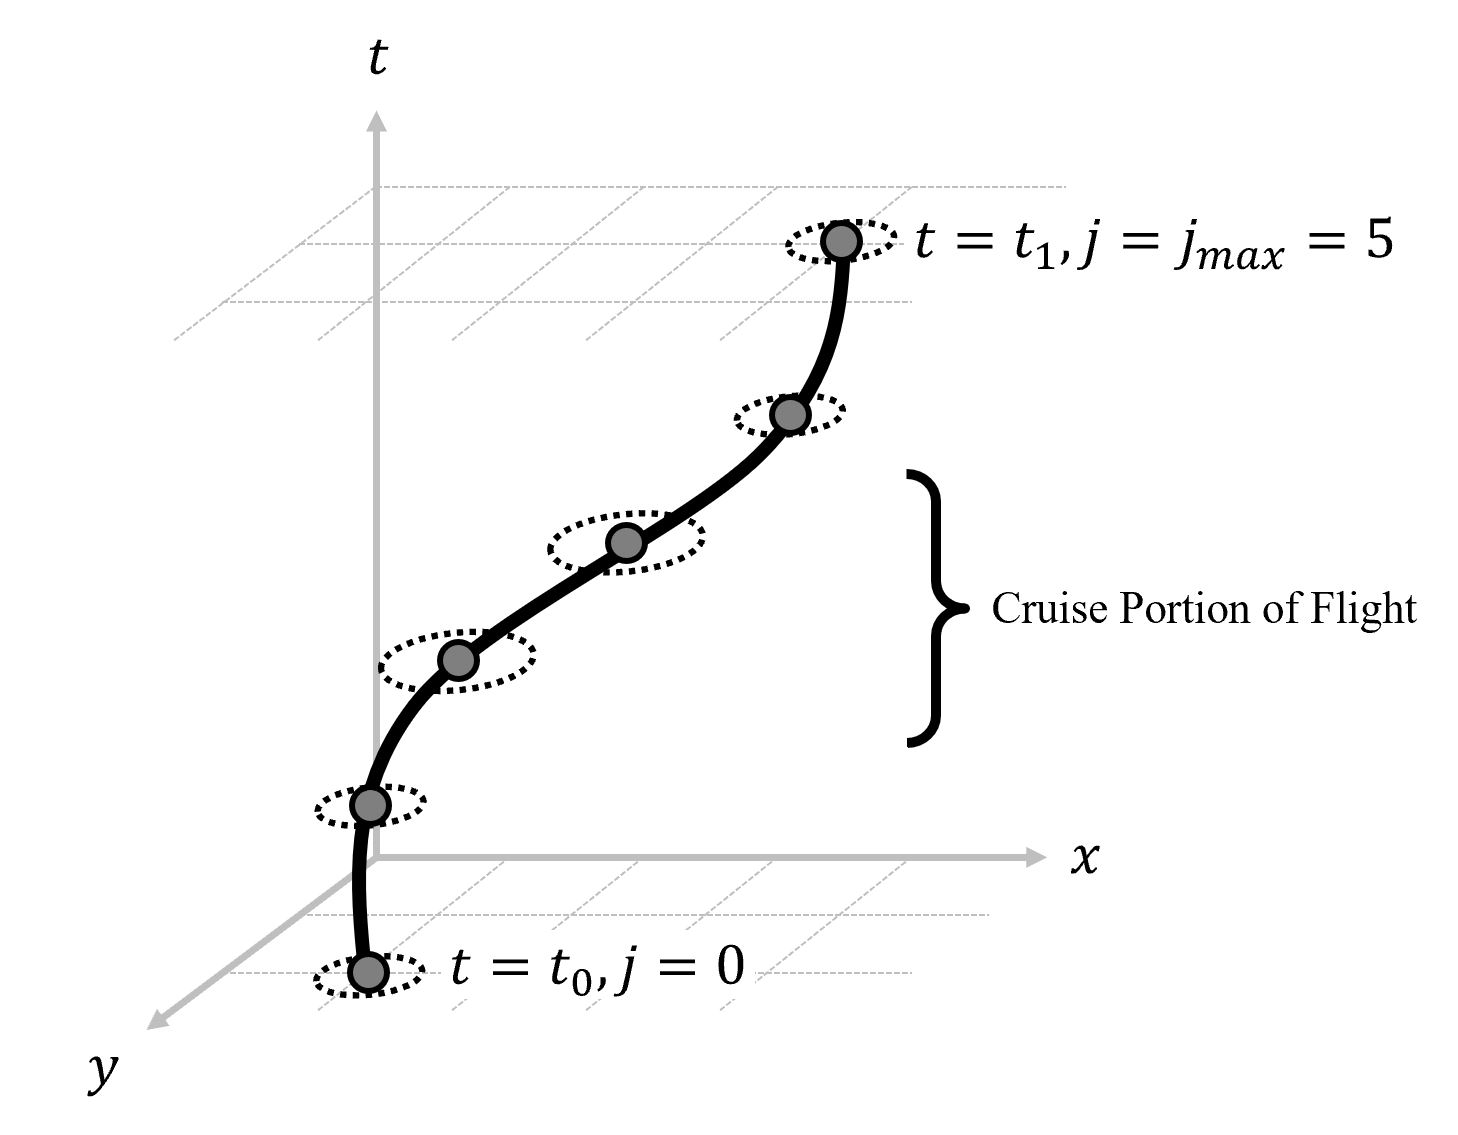
\includegraphics[width=0.8\textwidth]{figs/drone-path-concept}
\caption{Methodology's representation of a drone flying through space and time.}
\label{drone-path-concept}
\end{figure}

\begin{figure}[hbt!]
\centering
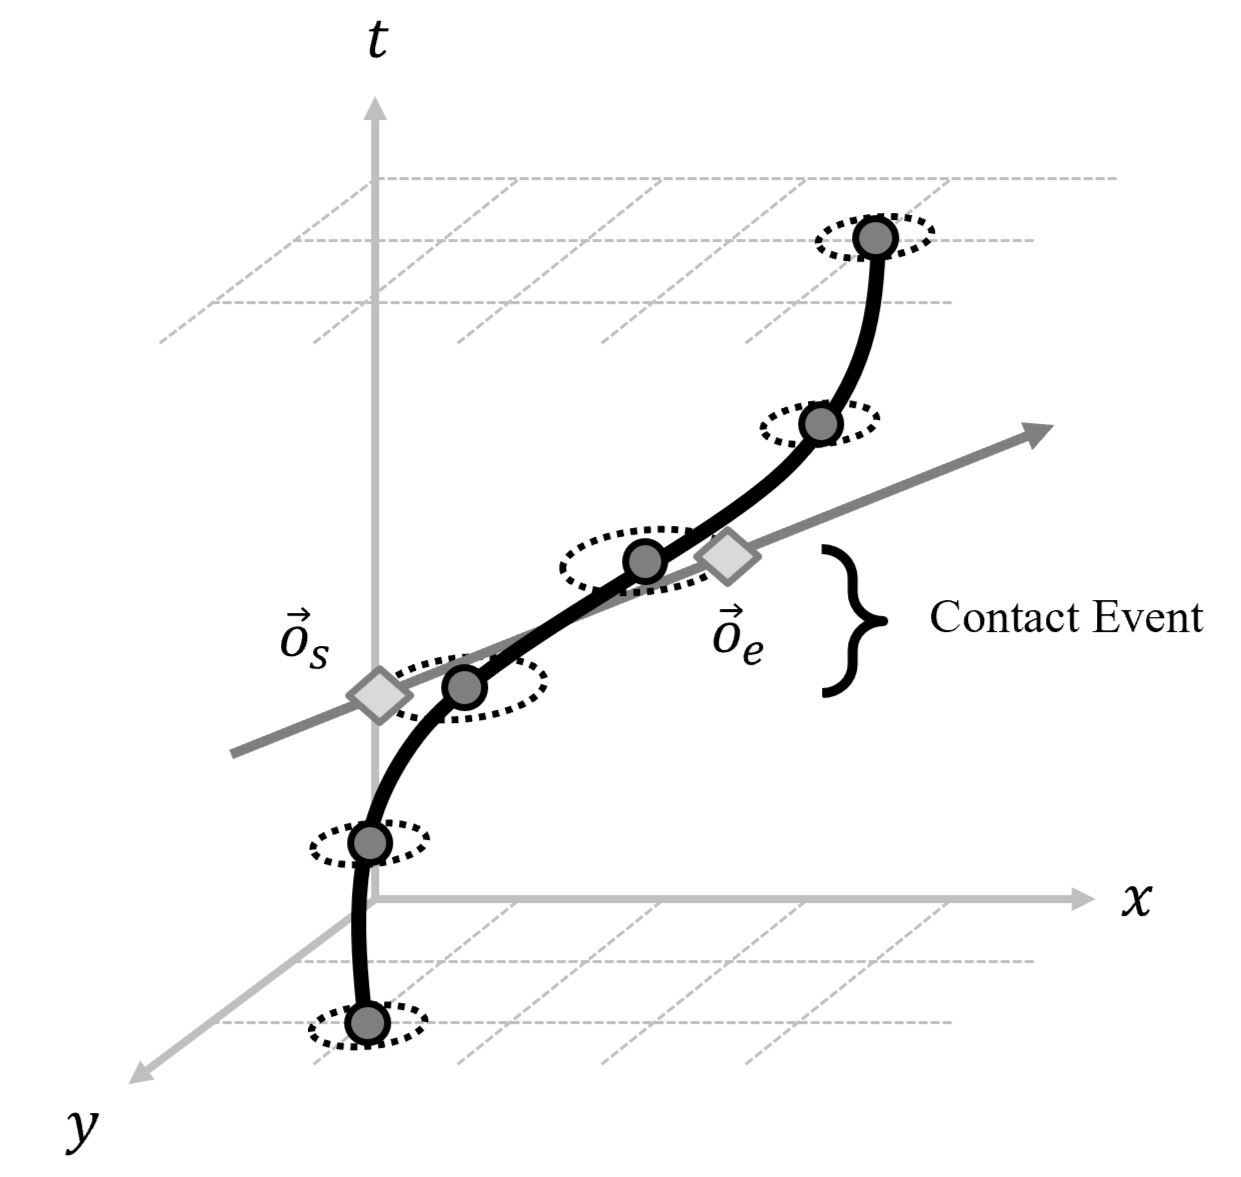
\includegraphics[width=0.7\textwidth]{figs/contact-event-concept}
\caption{Representation of contact event.}
\label{contact-event-concept}
\end{figure}

The methodology approaches the problem of object tracking by visualizing the entire system as a 3-dimensional volume shown in Fig. \ref{drone-path-concept}, where the $xy$-plane represents a region over which the drone fleet is to operate. In Fig. \ref{drone-path-concept}, the $z$-axis is the time-domain. As a result, drone flight paths and times of contact with the target object are visualized. 

With this 3-dimensional definition of drone and object, location vectors will be defined to represent the spatial location of the drone in the time-domain, in the form of $\vec{n}=[x, y, t]$, where $(x, y, t) \in (X, Y, T)$.

The sight parameter manifests itself as the radius of a thin circular slice parallel to the $xy$-plane. The small height (along the time axis) of this slice is equal to the time-step between each evaluated path node. Any simulated target object within this cylindrical volume is considered to have made ``contact'' with the manipulatable path node. This contact is referred to as a ``contact event'', being defined by the location/time of first contact and the last known location/time, as shown by Fig. (\ref{contact-event-concept}).



% ====================================================================
% METHODOLOGY
% ---------------------
% ====================================================================

\section{Methodology}

The following section outlines the methodology used to determine the optimal path alterations by means of a genetic algorithm. The algorithm and its user interface is run on a Flask server, which extracts and stores simulation data via connection to a MySQL database (structured query language database) hosted on the local machine. The source code can be found at \url{https://github.com/Leonardo767/aiaa2019-publication}, where everything except the static cascading styling sheets (for aesthetics) is original work of the author. Inside the source code sample folder, there are two main sections: ``lib'' and ``src'', which hold the code for application utilities and the genetic algorithm, respectively. For the script handling the application's data transfer and database connection, refer to ``routes.py''.


% A - Application Architecture
% ---------------------
\subsection{Application Architecture}
The application is run on a Flask server on the local machine. This was built to accelerate the development process by providing a means for the author to assess the incremental results generated by the optimization algorithm. The application was developed in the order of the workflow shown in Fig.~\ref{app-architecture}, beginning with the geographical data. This data contains information about the geography to be surveyed, such as the boundary dimensions, references to airports contained, and the  flight manifests referenced by said referenced airports. From here, flight paths can be constructed by extracting and manipulating the stored geographical information.

The next step is to input simulated objects. At the top level, the user can select simulation suites which represent the total movement of all objects for a given geographical region. It is important to note that this data is unknown to the fleet operator, and is only implemented here for the sole purpose of this \emph{simulated} data to act as an evaluation of the algorithm from an omniscient perspective. The individual objects themselves and their respective path points as a function of time can be edited within the MySQL database.

\begin{figure}[hbt!]
\centering
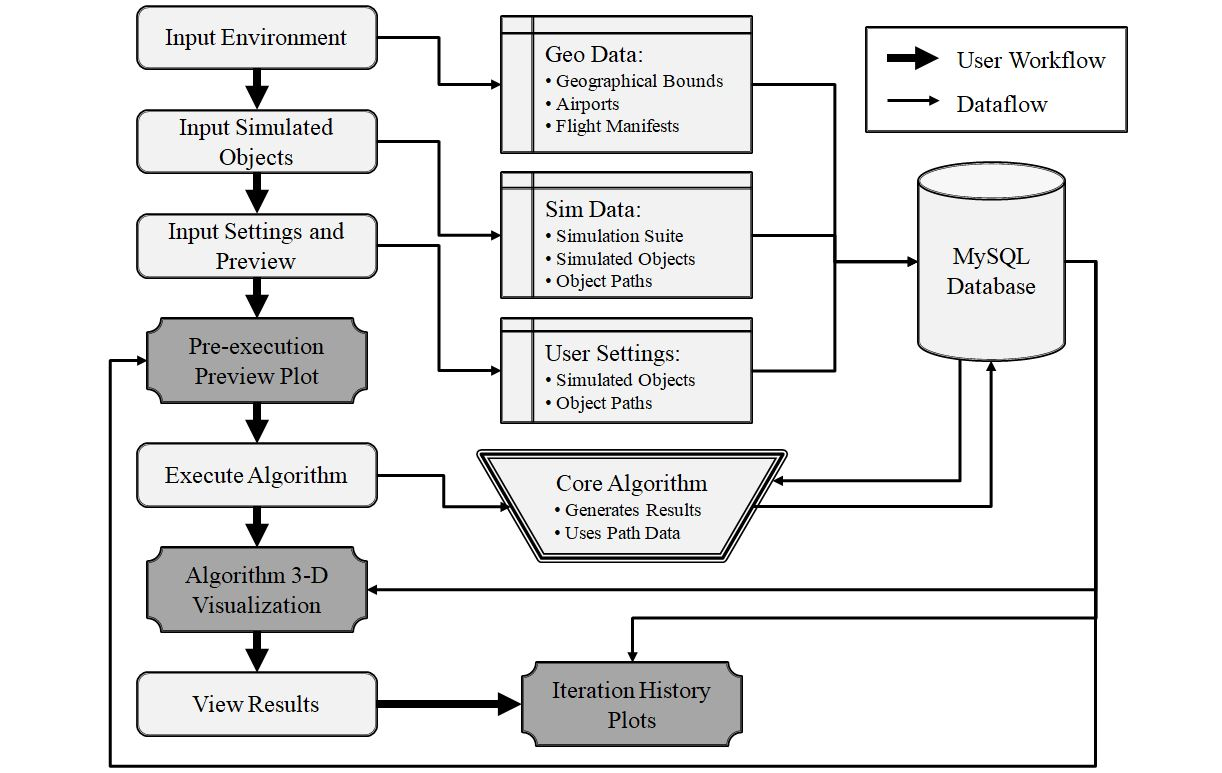
\includegraphics[width=1\textwidth]{figs/app-architecture}
\caption{Application architecture built to interface with core algorithm.}
\label{app-architecture}
\end{figure}

The settings input is used to add any additional simulation settings such as the load card used or fleet vehicle properties such as allowable velocity and range of sight. Within this page, an overall preview map is available of the region.

These data are fed into a MySQL database that the Flask app can interact with. It is from this database that the algorithm pulls information and packages its results per iteration. From these results, the plots of the altered paths are generated. Each database object's table holds references to other tables according to the structure shown in Fig. (\ref{db-structure}). The light-colored portions in italic font are associated with the simulation and are only used to compute the contact points. Again, the genetic algorithm is unaware of simulation data outside of what the contact event is composed of.

\begin{figure}[hbt!]
\centering
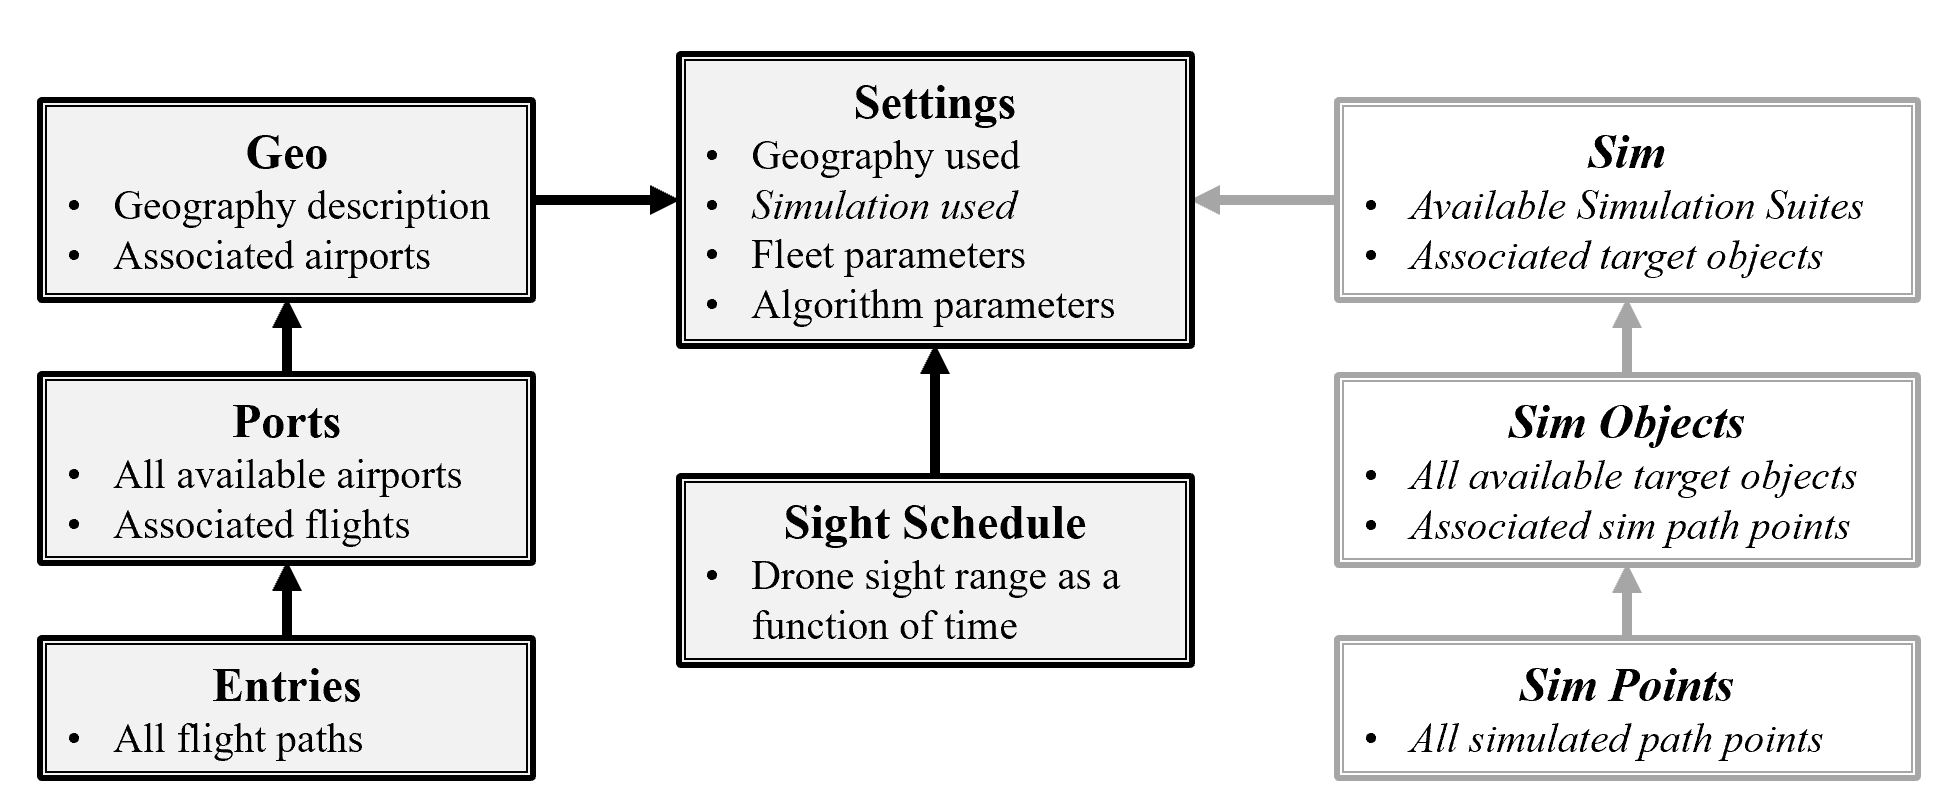
\includegraphics[width=1\textwidth]{figs/db-structure}
\caption{MySQL Database Structure for Application.}
\label{db-structure}
\end{figure}

The application then prompts the user to an execution page, where the number of iterations and type of execution is defined by one of four selected run-modes:
\begin{enumerate}
\item \emph{Reset}: resets iteration value and does one full iteration
\item \emph{Iteration++}: runs the next iteration
\item \emph{Execute Completely}: runs for iterations defined in execution settings
\item \emph{Debug (no plot)}: outputs via machine terminal, used for development
\end{enumerate}

Upon termination, the resulting altered fleet paths can be viewed in the 3-dimensional environment alongside the simulated paths. Additionally, historical plots are generated for the path alteration and parameter updates per iteration.


% B - Algorithm Architecture
% ---------------------
\subsection{Algorithm Architecture}
The algorithm is situated in the development application to mimic how it would operate in reality: the only information it interacts with is the known operational flight path and the simulated contact with the target objects. The fleet will fly its initial flight paths, and the coincidental contact made with the target objects (based on the sight parameter) provide the first iteration's input. The following sub-sections will further elaborate each labeled component in Fig.~\ref{algo-architecture}.

\begin{figure}[hbt!]
\centering
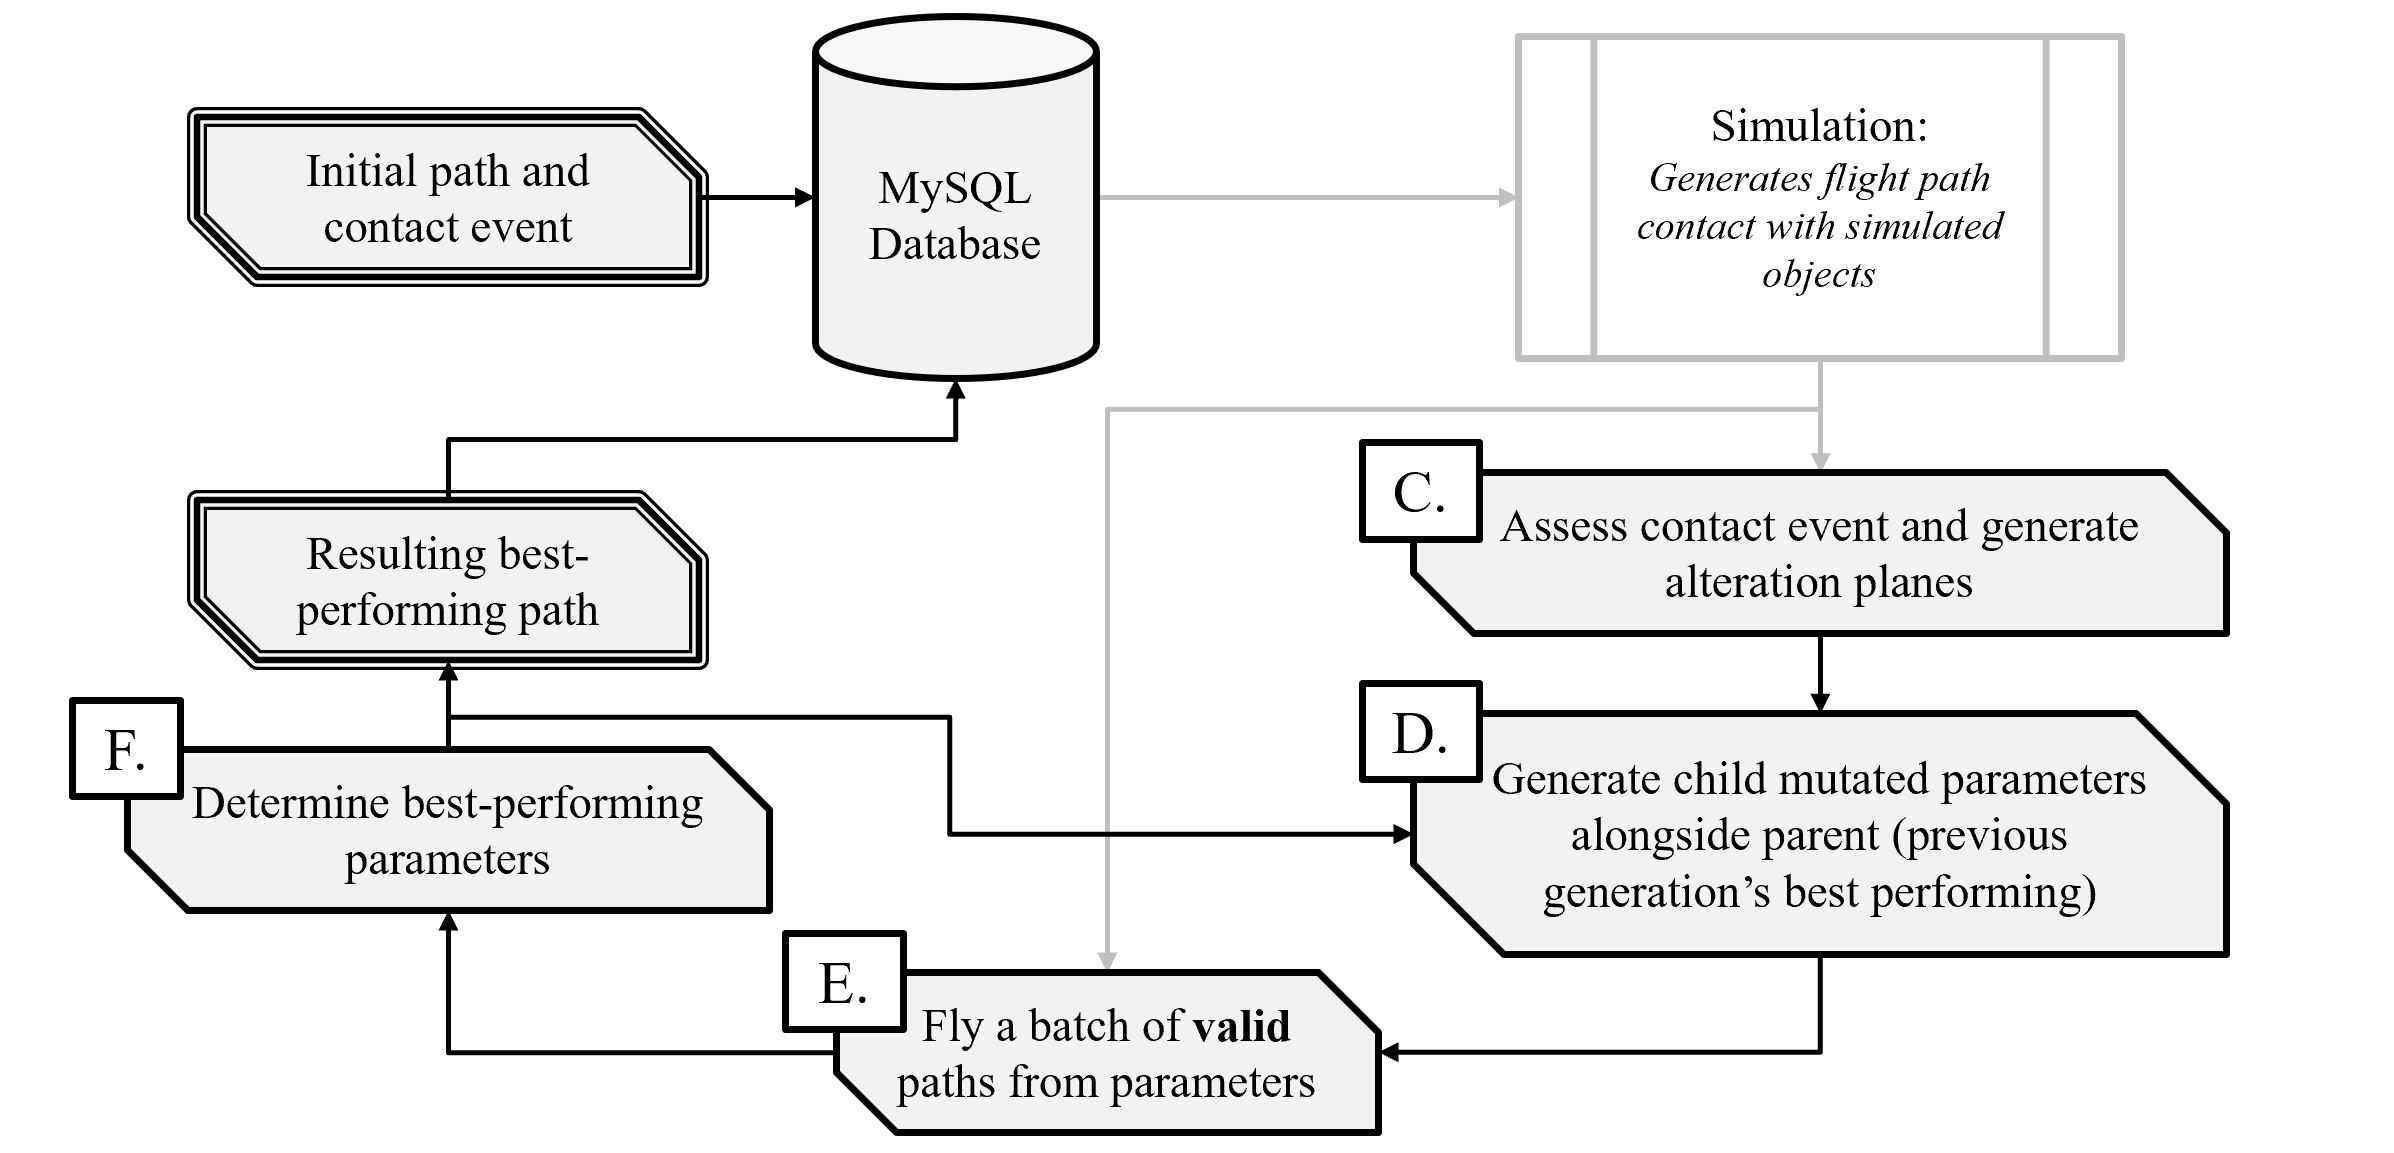
\includegraphics[width=1\textwidth]{figs/algo-architecture}
\caption{Top-level architecture of core algorithm.}
\label{algo-architecture}
\end{figure}


% C - Generating Alteration Planes
% ---------------------
\subsection{Assess Contact Event}

Upon the completion of a contact event, the situation is first described as two data objects in $\mathbf{R}^3$ space: the path of the simulated object and the path of the flight leg. Both are a collection of vectors describing the location of each path point.

For the generation of alteration vectors, only the points representing first and last contact are used, as these define the boundaries of the drone's observation (these points will be referred to as ``anchor points''). A collection of distance vectors is generated as the differences between the flight path vectors and anchor points using Eq. (\ref{d_vector}). Figure \ref{heuristic-diagram} shows this relationship between the flight path and tracked object.

\begin{equation}
\label{d_vector}
\vec{d}_{j_{\{s, e\}}} = \vec{o}_{\{s, e\}} - \vec{n}_j
\end{equation}

\begin{figure}[hbt!]
\centering
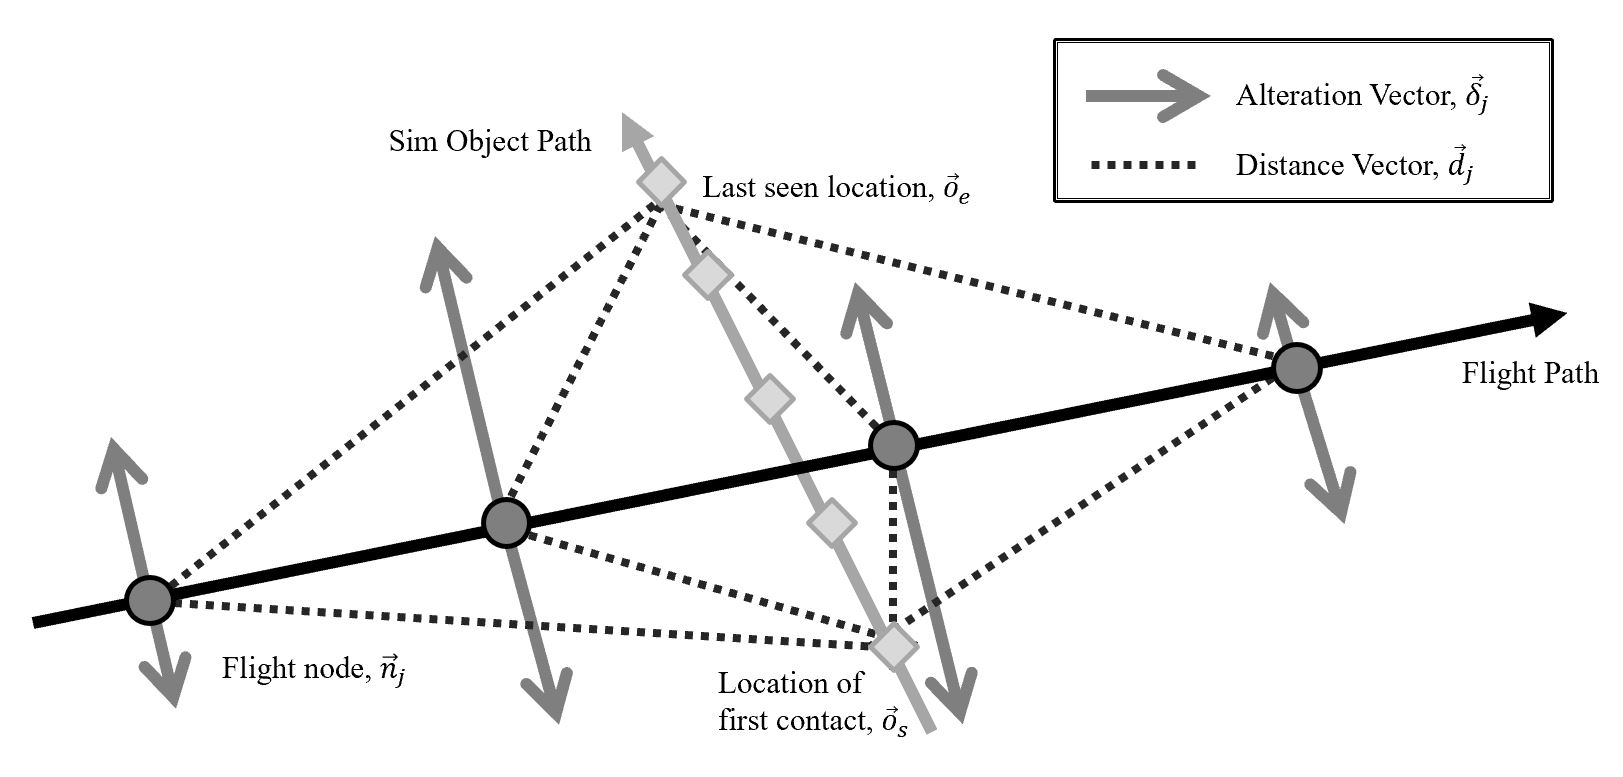
\includegraphics[width=1\textwidth]{figs/heuristic-diagram}
\caption{Relationship between flight and object path.}
\label{heuristic-diagram}
\end{figure}

It can be seen that $\vec{d}_j$ is divided by the set $\{s, e\}$. For each object point $\vec{o}_s$ and $\vec{o}_e$, a planar subspace is generated with basis vectors $\vec{d}_j$ and $(\vec{n}_{j + 1} - \vec{n}_j)$. From here, the Gram-Schmidt process is employed to generate an orthonormal basis using $(\vec{n}_{j + 1} - \vec{n}_j)$ as one of the basis vector directions. The basis vector normal to the plane is used as the direction for that node's alteration vector, keeping in mind that this is with respect to the object point $\vec{o}_{\{s, e\}}$. These basis vectors are computed by Eqs. (\ref{normal-basis1}) and (\ref{normal-basis2}), where the latter computes the direction of the alteration vector.

\begin{equation}
\label{normal-basis1}
\vec{u}_1 = \frac{\vec{n}_{j + 1} - \vec{n}_j}{\|\vec{n}_{j + 1} - \vec{n}_j\|}
\end{equation}

\begin{equation}
\label{normal-basis2}
\vec{u}_{2_{\{s, e\}}} = \frac{\vec{d}_{j_{\{s, e\}}} - \left(\vec{d}_{j_{\{s, e\}}}{\cdot}\vec{u}_1\right){\circ}\vec{u}_1}{\left\|\vec{d}_{j_{\{s, e\}}} - \left(\vec{d}_{j_{\{s, e\}}}{\cdot}\vec{u}_1\right){\circ}\vec{u}_1\right\|}
\end{equation}

Note that $\vec{u}_1$ is common to both $\{s, e\}$ planes. They only differ by the direction of the orthogonal vector $\vec{u}_2$, such that the common line of intersection between these two planes is the flight path itself.


% D - Generating Child Paths
% ---------------------
\subsection{Generating Child Paths}

For both planes, a set of alteration vectors are generated along $\vec{u}_2$ for each flight path node. The nodes are altered along each plane's second orthonormal basis using Eq. (\ref{node_update}).

\begin{equation}
\label{node_update}
\vec{n}_{j_{{\{s, e\}}}}' = \vec{n}_{j_{\{s, e\}}} + \delta_{j_{\{s, e\}}}\vec{u}_{2_{\{s, e\}}}
\end{equation}

The basis $\vec{u}_2$ (normal to the flight path) is scaled by $\delta_j$, a scalar value specific to each $\vec{n}_j$ per node index. Each $\delta_j$ is determined as a function of $j$, the node's index on the total flight path. This function (shown as Eq. (\ref{alteration}) is driven by three shaping parameters $\beta$, $\sigma$, and $\mu$. This function takes on the shape of the normal distribution (scaled by $\beta$) to allow for a distinct, flexible peak deviation and gradual decline to zero deviation at both ends (the fixed flight path points).

\begin{equation}
\label{alteration}
\delta_{j_{\{s, e\}}} = \frac{\beta_{\{s, e\}}}{\sqrt{2\pi\sigma_{\{s, e\}}^2}}\exp\left({-\frac{{\left(j - \mu_{\{s, e\}}\right)}^2}{2\sigma_{\{s, e\}}^2}}\right)
\end{equation}

The shape of each alteration set is independent within its respective plane. After the alteration set is generated by Eq. (\ref{node_update}) for each plane, the sets are merged into one new path by averaging the alteration vectors. The degree to which a node will be influenced by an alteration plane is weighted by a node's distance to that plane's respective anchor point ($\vec{o}_s$ or $\vec{o}_e$) using Eq. (\ref{plane_blend}).

\begin{equation}
\label{plane_blend}
\vec{n}_j' = \frac{\|\vec{d}_{j_e}\|}{\|\vec{d}_{j_s}\| + \|\vec{d}_{j_e}\|}\vec{n}_{j_s}' + \left(1 - \frac{\|\vec{d}_{j_e}\|}{\|\vec{d}_{j_s}\| + \|\vec{d}_{j_e}\|}\right)\vec{n}_{j_e}'
\end{equation}

Note that the parameters $\beta$, $\sigma$, and $\mu$ are what define the shape of the $\vec{n}_j'$ nodes. To initialize these parameters, educated guesses are made to approximate a good fit based on the initial contact using the heuristic Eqs. (\ref{best_beta}), (\ref{best_sigma}), and (\ref{best_mu}).

\begin{equation}
\label{best_beta}
\vec{\beta}_{\{s, e\}_{i = 0}} = 16\min(\vec{d}_{\{s, e\}})
\end{equation}

\begin{equation}
\label{best_sigma}
\vec{\sigma}_{\{s, e\}_{i = 0}} = \frac{1}{16}j_{max}
\end{equation}

\begin{equation}
\label{best_mu}
\vec{\mu}_{\{s, e\}_{i = 0}} = j_{\min(\vec{d}_{\{s, e\}})}
\end{equation}

After initial parameters are heuristically selected, they are mutated slightly to form a batch of paths that can be attempted and assessed. The purpose of this is to eventually replace the old parameters with the best-performing of this batch. Because each attempted flight requires the passage of a cycle, the batches are kept small (no more than 10) for faster improvement. Depending on cycle times and time constraints, an operator may find it infeasible to take something like 20 flights for each iteration's batch. For continuous improvement, a batch size of 1 may be selected, but this may lead to settling at a local optimum rather than exploring for a better overall shape. The larger the batch size, the more exploratory the algorithm would be before selecting an optimal parent parameter to select from. For these reasons, a batch size of 8 was selected during the experiments.

According to the batch size, sets of randomly mutated shaping parameters $\beta_{b_{\{s, e\}}}'$, $\sigma_{b_{\{s, e\}}}'$, and $\mu_{b_{\{s, e\}}}'$ are generated from their parent using Eq. (\ref{parameter_mutate}). Note that $\mbox{randn}(B)$ is a PyTorch function which outputs $B$ normally distributed random numbers with a mean of 0 and standard deviation of 1.

\begin{equation}
\label{parameter_mutate}
{\{\beta, \sigma, \mu\}}_{\{s, e\}}' = {\{\beta, \sigma, \mu\}}_{\{s, e\}}\left(1 + \eta\left[\mbox{randn}(B)\right]\right)
\end{equation}

Once the batch of parameter sets are determined, the change to the each mutated set's path is computed per node as explained by Eqs. (\ref{node_update}), (\ref{alteration}), and (\ref{plane_blend}). With the resulting contact events from the modified path nodes $\vec{n}_j'$ driven by ${\{\beta, \sigma, \mu\}}_{\{s, e\}}'$, the performance of each path is now ready to be assessed.


% E - Flying Batch of Valid Paths
% ---------------------
\subsection{Flying Batch of Valid Paths}
\label{Flying-Batch-of-Valid-Paths}

Before flying each mutated path $\left[\vec{n}_j'\right]_b$, a flight must first be assessed to ensure that the proposed alterations are within the vehicle's flight envelope. This flight envelope, defined by parameters $v_{min}$ and $v_{max}$, will set constraints to node alterations as shown by Fig. (\ref{velocity-saturation}).

\begin{figure}[hbt!]
\centering
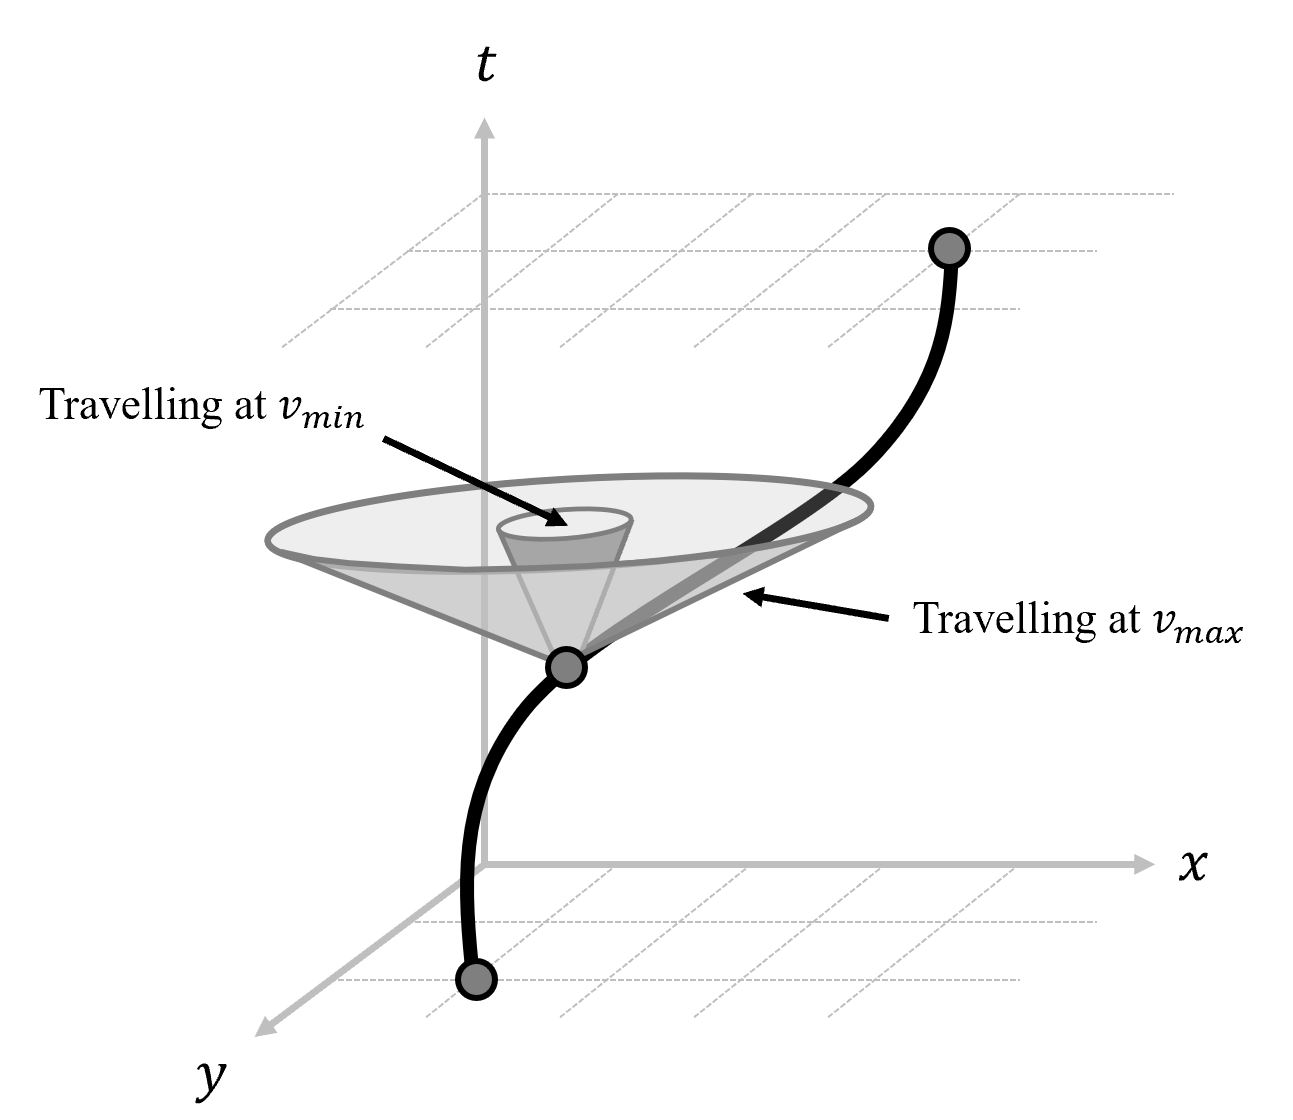
\includegraphics[width=0.75\textwidth]{figs/velocity-saturation-concept}
\caption{A flight path node bound by vehicle flight envelope}
\label{velocity-saturation}
\end{figure}

Conceptually, the cones of possibility in Fig. (\ref{velocity-saturation}) are a function of the flight envelope, where all points along possible paths will satisfy Eq. (\ref{vehicle-velocity}), which defines the velocity of a given drone in terms of the two spatial axes and time axis. This connects the fleet's vehicle constraints to the allowable path shape.

\begin{equation}
\label{vehicle-velocity}
v_{min} < \sqrt{\left(\frac{\partial{x}}{\partial{t}}\right)^2 + \left(\frac{\partial{y}}{\partial{t}}\right)^2} < v_{max}
\end{equation}

In the numerical implementation, for each node segment, a Boolean value is generated if Eq. (\ref{velocity-saturate}) holds true.

\begin{equation}
\label{velocity-saturate}
v_{min} < \frac{\sqrt{\left(\vec{n}[x]'_{j + 1} - \vec{n}[x]'_{j}\right)^2 + \left(\vec{n}[y]'_{j + 1} - \vec{n}[y]'_{j}\right)^2}}{\vec{n}[t]'_{j + 1} - \vec{n}[t]'_{j}} < v_{max}
\end{equation}

If all the nodes for a proposed path passed through Eq. (\ref{velocity-saturate}) return True, the path makes it into the batch to fly. If none of the parameters make it into an iteration's batch, a new set of proposed paths is generated with a more conservative mutation parameter. This continues until a proposed mutated path makes it into the flying batch or the number of attempts time out. If this time out happens, the algorithm terminates and requests that the user increase the margin between the original path and the flight envelope. For example, if a drone's original flight path is flying at its maximum velocity for the entirety of the cruise, any marginal alteration to the path with respect to the time axis would make that alteration invalid to fly.

% F - Determine Performance
% ---------------------
\subsection{Determine Performance}
Performance is determined by the percentage of the flight time where the drone is in contact with target object. The flight time is computed by Eqs. (\ref{building-valid-k}) and (\ref{performance-calc-equation}), or as Algorithm (\ref{find-contact-time}).

\begin{equation}
\label{building-valid-k}
\left\{k_{valid}\right\} = k \in K, \text{if } \left(\vec{o}_{k + 1}[t] - \vec{o}_k[t] < t_{min}\right) \text{ \& } \left(k \neq k_{max}\right)
\end{equation}

\begin{equation}
\label{performance-calc-equation}
P_b = \frac{1}{\left[\vec{n}[t]_{j_{max}} - \vec{n}[t]_{j_{min}}\right]}\sum\limits_{k=\left\{k_{valid}\right\}}t_k
\end{equation}

\begin{algorithm}
\textbf{INPUT:} Discovered contact event nodes for child $\left[\vec{o}_k\right]_b$; total flight time $\vec{n}[t]_{j_{max}} - \vec{n}[t]_{j_{min}}$.\\
\textbf{OUTPUT:} Performance for child $P_b$.
\begin{algorithmic}
\STATE Contact Time $t_K = 0$
\STATE Continuous contact threshold $t_{min}$
\FORALL{$k$ in $(0, K.length - 1)$}
\IF{$\vec{o}_{k + 1}[t] - \vec{o}_k[t] < t_{min}$}
\STATE $t_K = t_K + \vec{o}_{k + 1}[t] - \vec{o}_k[t]$
\ENDIF
\ENDFOR
\STATE Performance $P_b = t_K/\left[\vec{n}[t]_{j_{max}} - \vec{n}[t]_{j_{min}}\right]$
\end{algorithmic}
\caption{Calculating Performance for a Mutated Path $\left[\vec{n}_j'\right]_b$}
\label{find-contact-time}
\end{algorithm}

The parameters ${\{\beta, \sigma, \mu\}}_b$ associated with $\max({P_b})$ will be the parent parameter set for the next iteration. Also, a mutation of the original informed parameters $\{\beta_0, \sigma_0, \mu_0\}$ will continuously have one child slot reserved in the batch. This ensures that there is a second, informed point of reference from which a high-performing child-path might arise. After many iterations, however, this ``oddball'' child spawned from the original parameters is unlikely to perform better than its highly-evolved counterparts. However, in the beginning, having this second opinion ensures that all the children don't stagnate at one local point of high performance.

The continuous contact threshold $t_{min}$ is defined as the amount of time for which two adjacent instances of contact with a target object are counted as continuous. For a given path, the drone may come into contact with the target multiple times. The running sum $t_K$ is kept to tally only the instances where the object is continuously observed for a given amount of time. This process is shown conceptually in Fig. (\ref{performance-calc}).

\begin{figure}[hbt!]
\centering
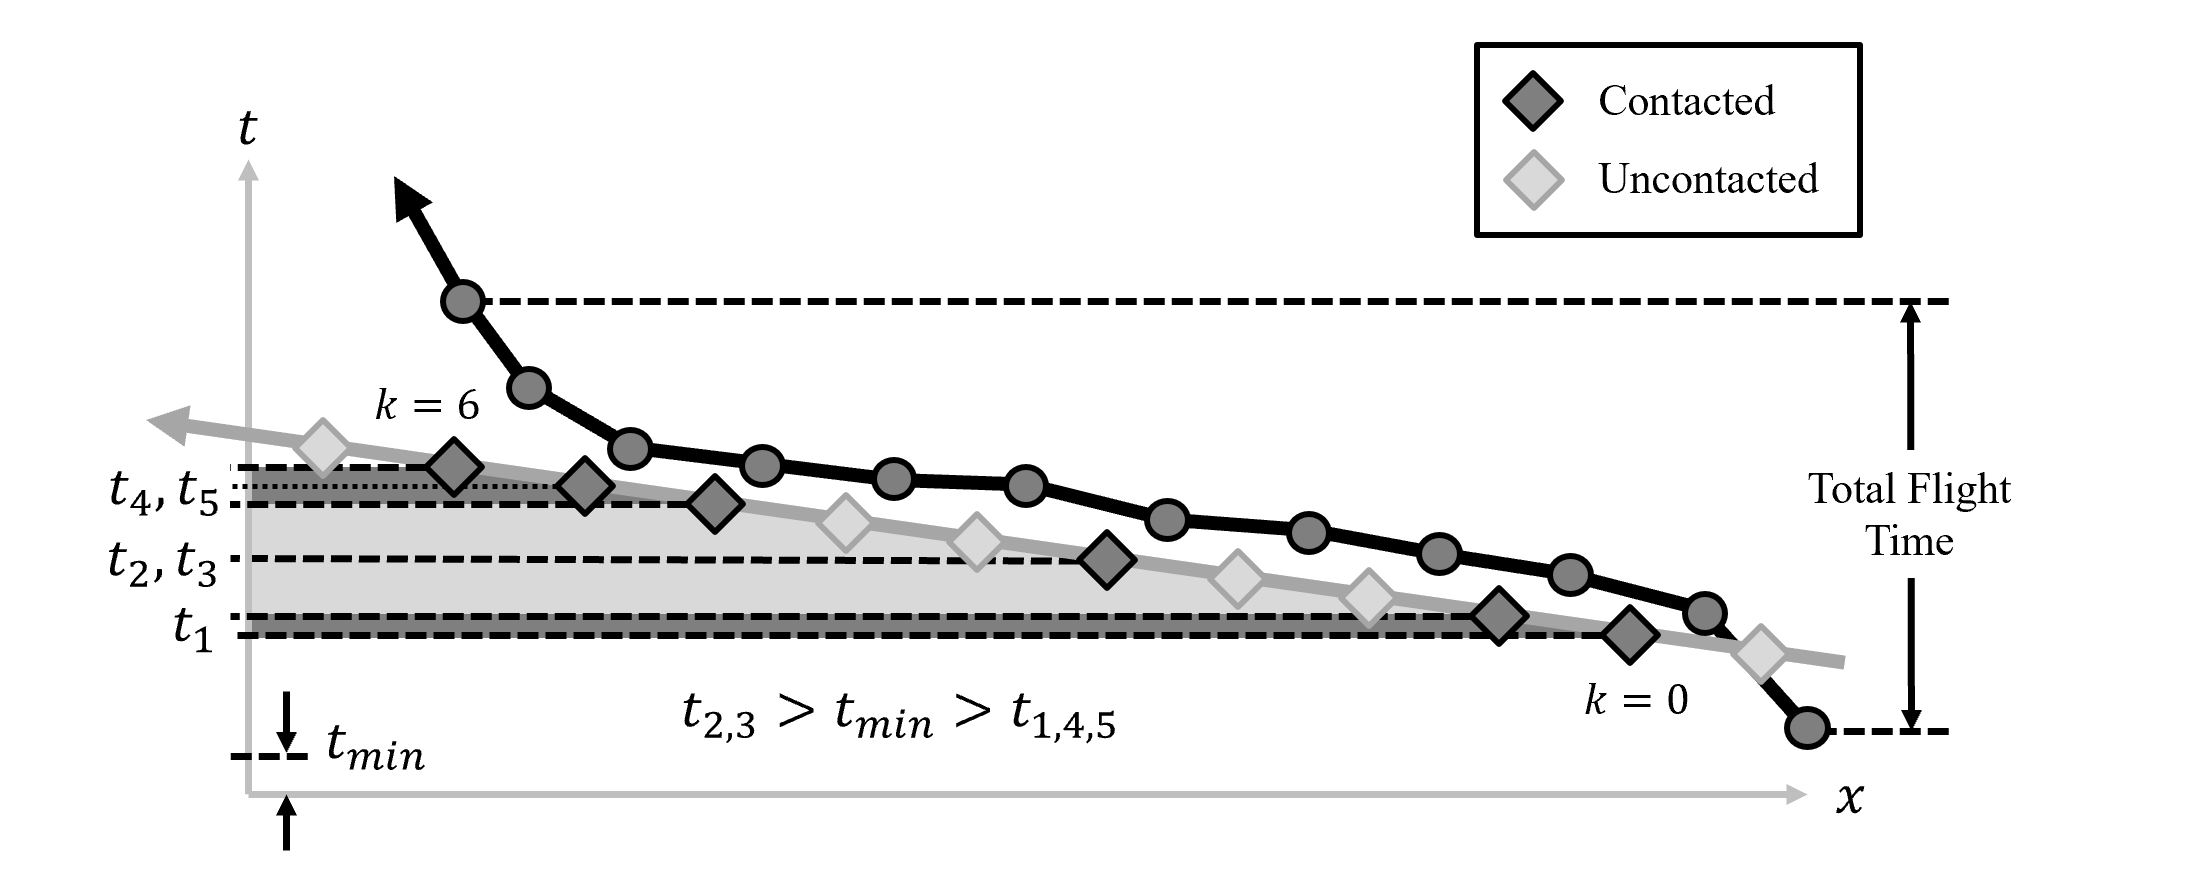
\includegraphics[width=1\textwidth]{figs/performance-calc}
\caption{Conceptual diagram for calculating $P_b$.}
\label{performance-calc}
\end{figure}


% G - Dynamic Hyperparameters
% ---------------------
\subsection{Dynamic Hyperparameters}
The optimum may be reached faster by increasing the mutation factor $\eta$. However, a large $\eta$ will likely deviate the path more than necessary. Additionally, the resulting large alterations to the original path are more likely to generate invalid proposed paths outside of the flight envelope.

On the other hand, an $\eta$ which is too small will require many iterations or flyable batches to significantly increase performance. In practice, this may be too expensive or outside of survey schedules.

The correct $\eta$ must be selected as a response to certain conditions. If performance has not significantly improved between iterations, $\eta$ is doubled. Otherwise, $\eta$ is decayed by a factor of 0.8 per successful iteration until it reaches one fifth of the original value. This continues until the minimum allowable $\eta$ is reached.

Within an iteration, if a proposed batch does not contain any flyable proposed paths, $\eta$ is lowered to generate more conservative paths. This is discussed at the end of subsection E.












\iffalse

% OLD STUFF
% ===================================================
% ===================================================
% ===================================================

\subsection{Old Stuff (ignore)}
\subsubsection{Assessing Contact Points}
Upon receiving information about the instances of contact with the target object, the first operation is to assess some basic properties about this event. These are inputs required to inform a devised heuristic. For each flight leg, the first and last seen location of the sim object is recorded. These two points serve as anchoring points for distance vectors created between these two locations and the locations of each path node. The alteration vector for each node will be determined from the components of each node's two respective distance vectors, as shown in Fig.~\ref{heuristic-diagram}.


For each node, the weighted sum of the two anchored vectors will drive its new location for the next iteration of the path. Said weighting will be determined by tuned parameters. For each iteration $i$, the determination of this alteration vector is of size $n$ and is defined in Eq. (\ref{change_vector_eqn}).

\begin{equation}
\label{change_vector_eqn}
\vec{n}_{i + 1} = \vec{n}_i + \vec{{\Delta}{n}}_i = \vec{n}_i + {\vec{\delta}}_i\circ{\vec{d}}_i = \vec{n}_i + \left({\vec{\delta}_{d_s}}\circ{\vec{\delta}_{d_e}}\circ{\vec{\delta}_{\theta_s}}\circ{\vec{\delta}_{\theta_e}}\circ{\vec{\delta}_j}\right)_i^T\circ{\vec{d}}_i
\end{equation}

Each of the Hadamard factors of $\delta$ is determined from Eqs. (\ref{delta_d_se_eqn}), (\ref{delta_theta_se_eqn}), and (\ref{delta_n_eqn}). The parameters $d$, $\theta$, and $j$ for each node are based on the contact event with the sim object and are described in the nomenclature.

\begin{equation}
\label{delta_d_se_eqn}
\vec{\delta}_{d_{\left\{s,e\right\}}} = \left[\frac{1}{\sqrt{2\pi{\sigma_{d_{\left\{s,e\right\}}}^2}}}\exp\left({-\beta_{d_{\left\{s,e\right\}}}\frac{{\left(\|{\vec{d}}\| - \mu_d\right)}^2}{2\sigma_{d_{\left\{s,e\right\}}}^2}}\right)\right]^{\vec{\rho}}
\end{equation}

\begin{equation}
\label{delta_theta_se_eqn}
\delta_{\theta_{\left\{s,e\right\}}} = \left[\frac{1}{\sqrt{2\pi\sigma_{\theta_{\left\{s,e\right\}}}^2}}\exp\left({-\beta_{\theta_{\left\{s,e\right\}}}\frac{{\left(\theta - \mu_\theta\right)}^2}{2\sigma_{\theta_{\left\{s,e\right\}}}^2}}\right)\right]^{\vec{\rho}}
\end{equation}

\begin{equation}
\label{delta_n_eqn}
\delta_j = \left[\frac{1}{\sqrt{2\pi\sigma_n^2}}\exp\left({-\beta_j\frac{{\left(j - \mu_j\right)}^2}{2\sigma_j^2}}\right)\right]^{\vec{\rho}}
\end{equation}

Eqs. (\ref{delta_d_se_eqn}), (\ref{delta_theta_se_eqn}), and (\ref{delta_n_eqn}) are all shaping functions for their respective property parameters, taking the form of a normal distribution about $0$ or $\frac{\pi}{2}$. They are also scaled by a tuned $\beta$ and $\sigma$. Through several iterations, optimally tuning the relationships between these driving parameters is what allows $\vec{{\Delta}{n}}_i$ to be intelligently determined.

It is important to note that the $\delta$ weights can be asymmetric with respect to which sim object endpoint $\{s,e\}$ they anchor to. This allows for the algorithm to create optimal ``S''-shapes in order to better track an object moving perpendicular to the flight path, as illustrated in Fig.~\ref{heuristic-diagram}. Otherwise, the nodes would cluster near the center, where its two alteration vectors would cancel from each anchor point, drawing the node to the midpoint of the two anchor points. This does not matter for a contact event where the object is moving parallel to one side of the flight, since the starting conditions are asymmetric and both anchor points draw the path towards whatever side of the flight path they happen to be on.

\subsubsection{Compute Resulting Cost}
To optimally tune these parameters, an evaluation function is required. There are two undesirable behaviors regarding alterations: deviation from the original path, which was known since defining the problem, and the tendency for nodes to cluster at one point (as if the alteration vectors create a sort of ``gravity'' about some resulting center point). The deviation is determined as the average distance from the original scheduled path using Eq. (\ref{path_deviation_eqn}), which would like to be minimized. 

\begin{equation}
\label{path_deviation_eqn}
C_{deviation_i} = \frac{1}{j_{max} - j_{min}}\sum\limits_{j=j_{min}}^{j_{max}}\frac{\|\vec{n}_{i_j} - \vec{n}_{0_j}\|}{\|\vec{n}_{0_{j_{min}}} - \vec{n}_{0_{j_{max}}}\|}
\end{equation}

The clustering is minimized by assigning a cost for inter-node distance having a standard deviation above zero, as determined by Eq. (\ref{internode_std_eqn}).

\begin{equation}
\label{internode_std_eqn}
C_{internode_i} = \sqrt{\frac{1}{j_{max} - j_{min}}\sum\limits_{j=j_{min}}^{j_{max} - 1}\left(\|\vec{n}_{i_j} - \vec{n}_{i_{j + 1}}\| - \overline{\|\vec{n}_{i_j} - \vec{n}_{i_{j + 1}}\|}\right)^2}
\end{equation}

A desirable behavior resulting from an alteration would be an increase in the length of time a simulated object can be observed by the new path. Since this is being used to determine a cost function to \emph{minimize}, the percentage of flight time during which the object is unseen factors into the cost using Eq. (\ref{contact_eqn}).

\begin{equation}
\label{contact_eqn}
C_{contact_i} = 1 - \frac{\vec{o}[t]_{i_{e}} - \vec{o}[t]_{i_{s}}}{\vec{n}[t]_{i_{j_{max}}} - \vec{n}[t]_{i_{j_{min}}}}
\end{equation}

To determine the total cost of this iteration, three positive hyper-parameters are required. These are hand-tuned according the relative importance of each undesirable behavior and determine the total cost using Eq. (\ref{total-cost}).

\begin{equation}
\label{total-cost}
C_i = \lambda_{deviation}C_{deviation_i} + \lambda_{internode}C_{internode_i} + \lambda_{contact}C_{contact_i}
\end{equation}


\subsubsection{Update Tuning Parameter Vector}
Upon determining the cost of the new contact event as a result of the $\beta$ and $\sigma$ parameters, the algorithm parameters can now be optimized according to Eq. (\ref{gradient-descent}),  a well-known equation in the subject of optimization.

\begin{equation}
\label{gradient-descent}
\left\{\beta, \sigma, \mu, \vec{\rho}\right\}_{i + 1} = \left\{\beta, \sigma, \mu, \vec{\rho}\right\}_i - \alpha\left(\frac{\partial{C_{i + 1}}}{\partial{\left\{\beta, \sigma, \mu, \vec{\rho}\right\}_i}}\right)
\end{equation}


\subsubsection{Tuned Path Alteration}
The main loop is continued by updating the node vector by the same Eq. (\ref{change_vector_eqn}), but instead using the updated parameters. After the nodes are updated, each alteration is saturated, if applicable, by any physical velocity limitations before committed. In this way there are no large jumps in position within a small timeframe. Higher-order acceleration and jerk saturation limiters may also be considered, but the time steps taken by the nodes seem to be large enough to reasonably assume that such criteria are met.

After the node locations are updated, this becomes the starting point for the next iteration. The main loop for updating node locations while actively tuning the parameters is summarized in Algorithm (\ref{algo:relgraph}).

\begin{algorithm}
\textbf{INPUT:} Object point locations continuously discovered by sim $\vec{o}_i$; initial flight path nodes $\vec{n}_0$; number of iterations $I$\\
\textbf{OUTPUT:} Final path nodes $\vec{n}_I$; final tuned shaping parameters $\left\{\beta, \sigma, \mu, \vec{\rho}\right\}_I$.
\begin{algorithmic}
\STATE Initialize variables to store history in database
\STATE Run simulation to create $\vec{o}_0$
\STATE Initialize dictionary of shaping parameters $\left\{\beta, \sigma, \mu, \vec{\rho}\right\}_0$ per flight leg
\FORALL{$i$ in $(1, I)$}
\STATE Run simulation to update $\vec{o}_i$ based on $\vec{n}_i$
\FORALL{flight in fleet paths}
\FORALL{path leg in flight}
\STATE Extract contacted points of leg in $\vec{o}_i$
\IF{contacted points exist}
\STATE Compute $\vec{\delta}_i, \vec{d}_i$ from $\vec{n}_i, \vec{o}_i, \left\{\beta, \sigma, \mu, \vec{\rho}\right\}_i$
\STATE Compute updated path $\vec{n}_{i + 1}$ from $\vec{n}_i, \vec{\delta}_i, \vec{d}_i$
\STATE Compute cost $C_{i + 1}$ from $\vec{n}_{i + 1}, \vec{o}_i, \left\{\beta, \sigma, \mu, \vec{\rho}\right\}_i$
\STATE Compute gradients of the cost with respect to $\left\{\beta, \sigma, \mu, \vec{\rho}\right\}_i$ using PyTorch auto-grad
\STATE Update shaping parameters $\left\{\beta, \sigma, \mu, \vec{\rho}\right\}_{i + 1}$ from gradients
\ENDIF
\STATE Store $\vec{n}_{i + 1}$ keyed by path leg
\STATE Store $\left\{\beta, \sigma, \mu, \vec{\rho}\right\}_{i + 1}$ keyed by path leg
\ENDFOR
\STATE Store path leg keyed by flight
\ENDFOR
\STATE Store fleet paths keyed by $i$
\ENDFOR
\end{algorithmic}
\caption{Main loop used to update flight path while tuning parameters}
\label{algo:relgraph}
\end{algorithm}




% \begin{table}
% \caption{\label{tab:table1} Transitions selected for thermometry}
% \centering
% \begin{tabular}{lcccccc}
% \hline
% & Transition& & \multicolumn{2}{c}{}\\\cline{2-2}
% Line& $\nu''$& & $J'' $& Frequency, cm$^{-1}$& $FJ$, cm$^{-1}$& $G\nu $, cm$^{-1}$\\\hline
% a& 0& P$_{12}$& 2.5& 44069.416& 73.58& 948.66\\
% b& 1& R$_{2}$& 2.5& 42229.348& 73.41& 2824.76\\
% c& 2& R$_{21}$& 805& 40562.179& 71.37& 4672.68\\
% d& 0& R$_{2}$& 23.5& 42516.527& 1045.85& 948.76\\
% \hline
% \end{tabular}
% \end{table}



% Visualization
% ---------------------
\subsection{Visualization}
Two plotting libraries were used to visualize the algorithm results of the simulation, and the overall aesthetics of the application consisted of imported Bootstrap templates. A large part of developing this algorithm involved the visualizations, since it provided feedback on whether a path was changing in the correct way. For example, in one trial, the path points were actually moving \emph{away} from the tracked object. From that observation, the problem was found to be a simple mistake in the calculation of the distance vector, which caused it to be pointing in the opposite direction. This mistake would have been difficult to detect so early on without a previously developed visualization.

All visualization data are extracted from the database so that the individual points do not need to be stored within the application's memory usage. Additionally, the MySQL workbench GUI allows for easy manipulation of data to test different cases. Before being processed by a plotting library, the data are stored in hash tables keyed by flight number and departure time. In this way, each flight leg has a unique set of data points and parameters to manipulate. This is done to allow the system to flexibly adapt to unique contact events, such as a perpendicular crossing, a crossing from the front left, or a parallel path on the right.

\subsubsection{Bokeh 2-D Plots}
The first plot displays the simulation setup before execution, showing a map of the paths taken by the target objects and fleet aircraft, as well as the location of airports (note that ``airports'' do not have to be airports, but can instead be fixed points in space where a vehicle must arrive at or depart from by a fixed time). 

The second plot is the unpacked plotted result for each iteration of paths generated by the algorithm.

\subsubsection{Plotly 3-D Plots}
This is the 3-dimensional interactive plot used to assess what the algorithm is processing per iteration.

\fi



% ====================================================================
% EXPERIMENTS
% ---------------------
% ====================================================================

\section{Experiments}

\subsection{Introductory 2-D Example}
On static, non-interactive images, it is difficult for a reader to interpret the plotted 3-D space. For this reason, the results of a 2-D pseudo-experiment are shown here. The purpose of this subsection is to provide context and introduce the reader to the plotted results of the following sections.

Suppose there are two locations in a fictional 1-dimensional geography, called $x_A$ and $x_B$. Both the simulated target and the drone are travelling from $x_A$ to $x_B$. The drone is travelling faster than the target, so while the target did depart at an earlier time, it arrived later than the drone. The resulting interaction between the drone and target is plotted in Fig. ().

Upon first contact, the the anchor nodes are chosen and distance vectors for each node are created. An orthonormal basis is created for each plane anchored by $\{\vec{o}_s, \vec{o}_e\}$, as illustrated by Fig. (). Note, in this 2-D example, these two anchored planes are co-planar, but may not necessarily have the same basis. They have parallel bases since here since the paths are straight (the second basis vector is derived from a path segment direction).

Informed parameters are now chosen and mutated to create a batch of proposed paths. The paths which violate the flight envelope are eliminated, as shown in Fig. ().

The best-performing path is selected after flying the batch. From here, the parameters which created this path are mutated, and the iteration loop is continued.

\subsection{Straight Parallel Encounter}
The first 3-D experiment presented is an encounter with a target travelling along a similar path to that of the drone. The expectation is that the drone path should be modified so that it creates a slight S-curve to match the path of the target.

\subsection{Straight Perpendicular Encounter}
This next experiment was an encounter with an object travelling perpendicular to the flight path. The resulting altered path is expected to contain a sharp S-curve that attempts to capture whatever contact it can for a brief amount of time.



% ====================================================================
% FUTURE WORK
% ---------------------
% ====================================================================
\section{Future Work}
A genetic algorithm was selected due to the unpredictable, non-differentiable relationship between the mutated shaping parameters and the performance measure (which was the result of a simulation unknown to the algorithm). However, there is a known, differentiable relationship between these parameters (or associated node locations) and the path length used. While $\eta$ was scheduled so that the path deviation would not be too severe, the algorithm can be extended to directly optimize the best performing path for travel length on each iteration. Eqs. (\ref{path_deviation_eqn}) and (\ref{gradient-descent}) show the underlying process of this extension.

\begin{equation}
\label{path_deviation_eqn}
C_i = \frac{1}{j_{max} - j_{min}}\sum\limits_{j=j_{min}}^{j_{max}}\frac{\|\vec{n}_{i_j} - \vec{n}_{0_j}\|}{\|\vec{n}_{0_{j_{min}}} - \vec{n}_{0_{j_{max}}}\|} \text{ where } \vec{n}_{i_j} = f\left(\beta_i, \sigma_i, \mu_i\right)
\end{equation}

\begin{equation}
\label{gradient-descent}
\left\{\beta, \sigma, \mu\right\}_{i + 1} = \left\{\beta, \sigma, \mu\right\}_i - \alpha\left(\frac{\partial{C_i}}{\partial{\left\{\beta, \sigma, \mu\right\}_i}}\right), \text{ if } P_b\left(\beta, \sigma, \mu\right)_{i + 1} = P_b\left(\beta, \sigma, \mu\right)_{i}
\end{equation}

Figure (\ref{future-extension}) shows where the extension should be located in the current implementation. The extension should be run at the end of each generation (iteration). In this way, the shaping parameters are further optimized within the differentiable bounds before the next mutation. This conserves energy and unecessary wear-and-tear on the vehicle.

\begin{figure}[hbt!]
\centering
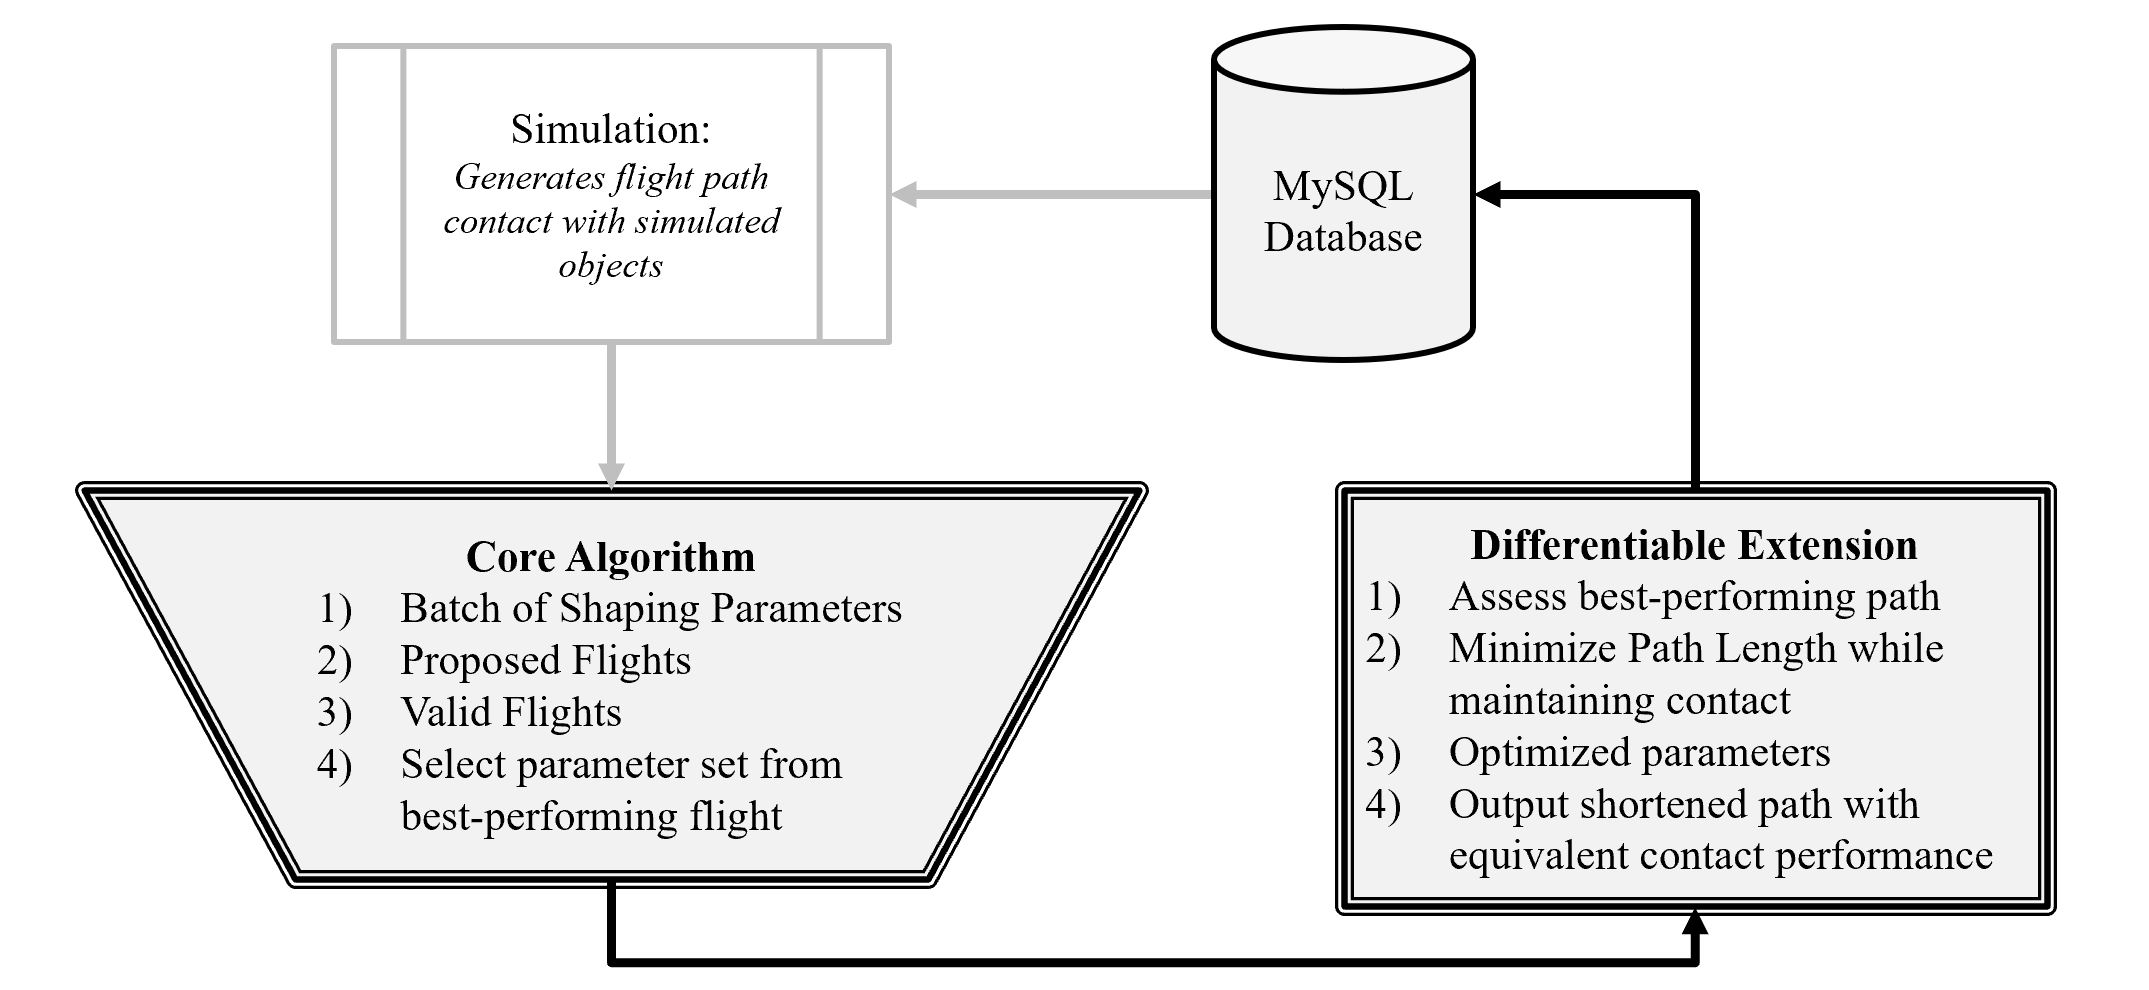
\includegraphics[width=1\textwidth]{figs/future-extension}
\caption{How proposed extension would interact with current implementation.}
\label{future-extension}
\end{figure}

One difficulty would be that this algorithm would create a slight disconnect between the shaping parameters and the resulting parent path, but genetic algorithms should be able to handle unknown circumstances anyway. Additionally, this extended differentiable algorithm will be bounded such that any optimized path must contain all the contact nodes.

The implementation of this extension is facilitated by the fact that all the node alteration operations described in this paper are conducted on PyTorch Tensor objects. A machine learning framework, PyTorch preserves information of the gradients for each forward operation as a computation graph. This preserved information is then used to automatically compute the gradients used to descend the cost function (path length).


% ====================================================================
% CONCLUSION
% ---------------------
% ====================================================================

\section{Conclusion}



% ====================================================================
% APPENDIX
% ---------------------
% ====================================================================

\section*{Appendix}


\section*{Acknowledgments}


\bibliography{sample}

\end{document}
